% This work by Jeremy A. Hansen is licensed under a Creative Commons 
% Attribution-NonCommercial-ShareAlike 3.0 Unported License, 
% as described at http://creativecommons.org/licenses/by-nc-sa/3.0/legalcode

Let's discuss strings.
Strings are a data type typically used to hold a collection of printable characters such as words, sentences, or longer sequences.
In order to use strings in your program you must first include the string library:

\noindent\begin{minipage}{\linewidth}\begin{lstlisting}
#include <string>
using namespace std;
\end{lstlisting}\end{minipage}

\noindent Also note that a string, for convenience, can be treated like an array of individual characters.

When we declare variables of type \Code{string}, we declare them just like we would an \Code{int}, \Code{float}, or \Code{double}.
We can create a variable named \Code{myString} of type string by doing this:

\noindent\begin{minipage}{\linewidth}\begin{lstlisting}
#include <string>
using namespace std;

string myString;
\end{lstlisting}\end{minipage}

\noindent If you choose not to have \Code{using namespace std;} in your code, the variable \Code{myString} must be declared as follows:

\noindent\begin{minipage}{\linewidth}\begin{lstlisting}
#include <string>

std::string myString;
\end{lstlisting}\end{minipage}

\noindent We can then store anything we want in that string as long as it is made up of characters.
When a literal value is assigned to a string, it should be surrounded by double quotes such as in the case of \Code{"Hello"}:

\noindent\begin{minipage}{\linewidth}\begin{lstlisting}
#include <string>

string myString = "Hello";
\end{lstlisting}\end{minipage}

If we are storing the value of a string entered by a user, the user does not have to use quotes.
We can store \Code{"Hello"} in the string by doing the following:

\noindent\begin{minipage}{\linewidth}\begin{lstlisting}
string myString;
cin >> myString; // User types: Hello
                 // myString is now "Hello"
\end{lstlisting}\end{minipage}

\noindent It is also possible to use the arithmetic operator \Code{+} with strings to concatenate (combine) the two strings.
If we combined one string that contained \Code{"Hello"} and another string that contained \Code{"World"} the connected string would then read \Code{"HelloWorld"}.

\noindent\begin{minipage}{\linewidth}\begin{lstlisting}
string v1 = "Hello",
       v2 = "World";
cout << v1 + v2 << endl;
// Outputs:
// HelloWorld
\end{lstlisting}\end{minipage}



In order to have a space between the two words, one of the strings would need to contain a space such as this:

\noindent\begin{minipage}{\linewidth}\begin{lstlisting}
string v1 = "Hello", v2 = " World";
//-------------------------^-------
cout << v1 + v2 << endl;
// Outputs:
// Hello World
\end{lstlisting}\end{minipage}

\noindent Or it can be represented as: 

\noindent\begin{minipage}{\linewidth}\begin{lstlisting}
string v1 = "Hello ", v2 = "World";
//----------------^----------------
cout << v1 + v2 << endl;
// Outputs:
// Hello World
\end{lstlisting}\end{minipage}

\noindent Alternatively, a space can be added like so: \nopagebreak[4]

\noindent\begin{minipage}{\linewidth}\begin{lstlisting}
string v1 = "Hello", v2 = "World";
cout << v1 + " " + v2 << endl;
//------------^-------------------
// Outputs:
// Hello World
\end{lstlisting}\end{minipage}

\noindent The first two concatenates the two strings to create one string that contains ``Hello World'', and the third concatenates three strings to produce the same result.

When reading strings from \Code{std::cin}, the default behavior is to collect all characters until the first whitespace (a tab, space, or newline) character that it finds in the input.
For example, if the user inputs ``Hello World'' in the following code, \Code{std::cin} stops reading at the first whitespace, and thus the string would contain only ``Hello''.
If we want to read the entire line of text, we need to use the \Code{getline()} function, which reads until the first newline character.
This is how you use the \Code{getline()} function:

\noindent\begin{minipage}{\linewidth}\begin{lstlisting}
string myString;
getline(cin, myString);
\end{lstlisting}\end{minipage}

\noindent This function call will take the entire line of input, including all whitespace characters, and store it in the variable \Code{myString}. 
		
We can also find out the length of the string by using the member function \Code{length()} with any \Code{string} object.
For example, if we wanted to find the length of a string entered by a user and store it in a variable named \Code{stringLength}, we might do this:

\noindent\begin{minipage}{\linewidth}\begin{lstlisting}
string myString;
int stringLength;
getline(cin, myString);
stringLength = myString.length();
cout << "The string you entered was "
     << stringLength
     << " characters long."
     << endl;
\end{lstlisting}\end{minipage}

\noindent Aside from finding the length of a string, we can search for certain characters in the string by using the \Code{find()} and \Code{rfind()} member functions.
For example, if we wanted to find a single space in a string variable named \Code{myString} that contains ``Hello World'', we would do this:

\noindent\begin{minipage}{\linewidth}\begin{lstlisting}
string myString = ;
int spot = myString.find(" ");
\end{lstlisting}\end{minipage}

This code results in the value 5 being stored in the variable named \Code{spot} because the space character is stored at index 5 if you treat the string as an array, as shown in Figure \ref{fig:string-diagram}.

\begin{figure}[t]
  \centering
  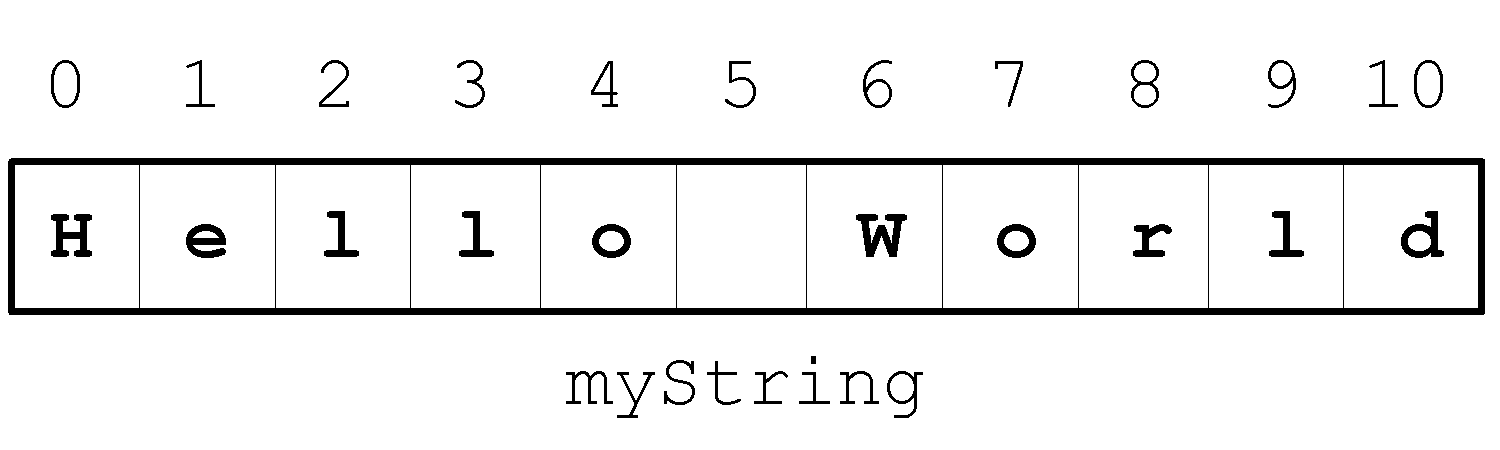
\includegraphics[width=0.7\textwidth]{diagrams/string-diagram.pdf}
  \caption{A \Code{string} viewed as an array} \label{fig:string-diagram} 
\end{figure}

Remember that we start at index 0, so even though the space is in the sixth position, it is at index 5 in the string.
When a line of text is stored in a string, think of it as being stored in memory in an array of the same length as there are characters in the string.
For example, the string \Code{"Hello World"} can be contained in an array with 11 slots, therefore the space character would be found in \Code{myString[5]}.
The \Code{find()} function can also search within a string from some arbitrary starting point, instead of from the beginning:

\noindent\begin{minipage}{\linewidth}\begin{lstlisting}
string myString = "Hello World";
int spot, spot2;
spot = myString.find(" "); // Found at index 5
// Starting from index 5, found at index 7
spot2 = myString.find("o", spot); 
\end{lstlisting}\end{minipage}

\noindent The second argument that is passed to the function (in this case, \Code{spot}) is the index at which you want to start your search.

We can also use the \Code{rfind()} function to find a character in reverse direction from the end of the string, or from some starting point, as above.
If we wanted to find the single character string \Code{"o"} before the space we might do something like this:

\noindent\begin{minipage}{\linewidth}\begin{lstlisting}
string myString = "Hello World";
int spot, spot2;
spot = myString.rfind(" "); // found at index 5
// starting from index 5, found at index 4
spot2 = myString.rfind("o", spot); 
\end{lstlisting}\end{minipage}

\noindent This function call to \Code{rfind()} uses the arguments \Code{"o"} and \Code{spot}.
This stores the position of the first \Code{"o"} it comes across after going in reverse from the index stored in \Code{spot} (which contains 5).
The last line would be equivalent to: \nopagebreak[4]

\noindent\begin{minipage}{\linewidth}\begin{lstlisting}
// starting from index 5, found at index 4
spot2 = myString.rfind("o", 5); 
\end{lstlisting}\end{minipage}

\noindent Both of these function calls will start searching for the string \Code{"o"} backwards from the same spot in the string, at index 5. 

Sometimes the string you search for cannot be found, as in this example:

\noindent\begin{minipage}{\linewidth}\begin{lstlisting}
string myString = "Hello World";
int spot = myString.find("Q"); // No Q in this string!
\end{lstlisting}\end{minipage}

\noindent In this case, the \Code{find()} (or \Code{rfind()}, for that matter) returns a special value named \Code{string::npos}.
When we use \Code{find()} or \Code{rfind()} and believe that they could fail, we should verify that the string was found, as below:

\noindent\begin{minipage}{\linewidth}\begin{lstlisting}
string userInput;
int spot;
cin >> userInput;
spot = userInput.find("Z");

if (spot == string::npos)
  cout << "There was no Z in what you typed!" << endl;
else
  cout << "The first Z was in position " << spot << endl;
\end{lstlisting}\end{minipage}
\LevelD{Review Questions}
\begin{enumerate}
\item Write code to declare a \Code{string} and take input from a user.
\item Can a \Code{string} be treated as a character array?
\item When do you use a \Code{string}?
\item What is the \Code{\#include} needed to use \Code{string}s?
\item What function do you have to use to take an input with a space?
\item Write code that takes in 5 words and outputs each of them 4 times.

\item Write a program that takes in the following words: King, Queen, Knight, Bishop, Rook, Pawn. 
Then it has to switch the King with the Pawn, the Rook with the Queen, and the Bishop with the Knight.
It must output the original data in the original order, and output the data once it is all finished.

\item Write a game program where the user inputs 4 different words, then the user gets 4 guesses to guess all of the words they originally Entered. This program should run as many times as the user wants.
\end{enumerate}

%\LevelD{Review Answers}

\LevelD{Further Reading}
\begin{itemize}
\item \url{http://www.harding.edu/fmccown/cpp_strings.pdf}
\item \url{http://www.stanford.edu/class/cs106x/handouts/08-C++-Strings.pdf}
\end{itemize}
